\documentclass[a4paper,twoside,12pt]{book}
%% === nezbytné balíčky:
\usepackage[T1]{fontenc}    % kódování písma
%\usepackage[IL2]{fontenc}  % kódování písma

\usepackage[utf8]{inputenc}     % vstupní znaková sada tohoto dokumentu: UTF-8
%\usepackage[cp1250]{inputenc}  % vstupní znaková sada tohoto dokumentu: Windows 1250
%\usepackage[latin2]{inputenc}  % vstupní znaková sada tohoto dokumentu: ISO Latin 2

\usepackage[english]{babel} % česky psaná práce, typografická pravidla. Překládejte pomocí "latex.exe" nebo "pdflatex.exe"
%\usepackage{czech} % česky psaná práce. Překládejte pomocí "pdfCSlatex.exe" ("cslatex.exe" asi bude mít problém s balíkem geometry)

\usepackage[a4paper, hmarginratio=3:2]{geometry} % využití A4 stránky a nastavení okrajů (u vazby bude širší)

\usepackage{pdfpages} % pokud nemáte formulář "Zadání bak./dipl. práce" naskenovaný jako PDF, tak ZAKOMENTUJTE
\usepackage[hidelinks]{hyperref} % v PDF budou klikací odkazy ("hidelinks" je nebude rámovat)

 \hypersetup{
     colorlinks=true,
     linkcolor=blue,
     filecolor=blue,
     citecolor = black,      
     urlcolor=cyan,
     }

%% === balíčky, které se mohou hodit:
%\usepackage{encxvlna} % postará se o spojky a předložky, které dle českých pravidel nesmí být na konci řádku. Dokumentace: http://texdoc.net/texmf-dist/doc/generic/encxvlna/encxvlna.pdf (chová se správně k "vnitřku" listings?)

\usepackage{graphicx} % balíček pro vkládání rastrových grafických souborů (PNG apod.)
%\usepackage{epsfig} % balíčky pro vkládání grafických souborů typu EPS
%\usepackage{float} % rozšířené možnosti umístění obrázků

%\usepackage{caption} % pro popisky obrázků, tabulek atd.

\usepackage{tabularx} % rozšířené možnosti tabulek
%\usepackage{tabu} % jiný balík pro rozšířené možnosti tabulek

%\usepackage{listings}  % balíček vhodný pro ukázky zdrojového kódu v~textu práce/příloh. Nutno nastavit! http://ftp.cvut.cz/tex-archive/macros/latex/contrib/listings/listings.pdf
\usepackage{amsmath} % balíček pro pokročilou matematickou sazbu
%\usepackage{color} % pro možnost barevného textu
%\usepackage{fancybox} % umožňuje pokročilé rámečkování

%\usepackage{index} % nutno použít v případě tvorby rejstříku balíčkem makeindex
%\newindex{default}{idx}{ind}{Rejstřík} % zavádí rejstřík v případě použití balíku index

\usepackage{epigraph}
%\ setting the epigraph width
\setlength{\epigraphwidth}{0.8\textwidth}


% Biblatex package for references
\usepackage[sorting=none]{biblatex}
\addbibresource{sample.bib}

% For headers and footers
\usepackage{fancyhdr}

\pagestyle{fancy}
\renewcommand{\chaptermark}[1]{\markboth{#1}{#1}}
\fancyhead[R]{}
\fancyhead[L]{}
\fancyfoot[C]{\thepage}


% path for figures
\graphicspath{{img/}}

% for footnotes in tables
\usepackage{booktabs,caption}
\usepackage[flushleft]{threeparttable}

% for table footnotes and captions
\usepackage{caption}
\usepackage{subcaption}

% for code highlightning
\usepackage{minted}

% for Appendixes
\usepackage[toc,page]{appendix}

% for nomenclature
\usepackage{nomencl}
\makenomenclature

% for printing of units
\usepackage{siunitx}
\sisetup{load-configurations = abbreviations}

% for printing of multiline comments
\usepackage{verbatim}

% for glosaries and acronyms
\usepackage[acronym, toc]{glossaries}
\makeglossaries
\input{appendices/acronyms.tex}

\frenchspacing % za větou bude mezislovní mezera (v anglických textech je mezera za větou delší)
\widowpenalty=1000 % "síla" zákazu vdov (= jeden řádek ze začátku odstavce na konci stránky)
\clubpenalty=1000 % "síla" zákazu sirotků (= jeden řádek/slovo z konce odstavce samostatně na začátku stránky)
\brokenpenalty=1000 % "síla" zákazu zlomu stránky za řádkem, který má na konci rozdělené slovo


\topmargin=-15mm      % horní okraj trochu menší
\textwidth=150mm      % šířka textu na stránce
\textheight=240mm     % "výška" textu na stránce


\pagenumbering{arabic} % číslování stránek arabskými číslicemi


\parindent=0pt % odsazení 1. řádku odstavce
\parskip=7pt   % mezera mezi odstavci

\newcommand{\ti}{\textit} % zkrácený příkaz pro kurzívu
\newcommand{\tb}{\textbf} % zkrácený příkaz pro tučné písmo


%% --- zde jsou zavedeny některé "konstanty" - některé musíte změnit! --- %%
\newcommand{\cvut}{Czech Technical University in Prague}
\newcommand{\fjfi}{Faculty of Nuclear Sciences and Physical Engineering }
\newcommand{\program}{Applications of Natural Sciences}

\newcommand{\obor}{Physical engineering} % změňte, pokud máte jiný obor

\newcommand{\druh}{Study for dissertation} % nebo "Diplomová práce"
\newcommand{\woman}{} % pokud jste ŽENA, ZMĚŇTE na: ...{\woman}{a} (je to do Prohlášení)

\newcommand{\logoCVUT}{\includegraphics{img/symbol_cvut.pdf}} % logo ČVUT -- podle grafického manuálu ČVUT platného od prosince 2016. Pokud nevyhovuje PDF-verze, tak použijte jinou variantu loga: https://www.cvut.cz/logo-a-graficky-manual -> "Symbol a logo ČVUT v Praze"). Pokud chcete logo úplně vynechat, zadejte místo "\includegraphics{...}" text "\vspace{35mm}"

% přesně podle formuláře "Zadání bak./dipl. práce" VYPLŇTE:
\newcommand{\nazevcz}{Postprocesor robota pro metodu Laser Shock Peening}    % český název práce (přesně podle zadání!)
\newcommand{\nazeven}{Robot post processor for Laser Shock Peening technique}          % anglický název práce (přesně podle zadání!)
\newcommand{\autor}{Marek Böhm}   % vyplňte své jméno a příjmení (s akademickým titulem, máte-li jej)
\newcommand{\vedouci}{Ing. Josef Blažej, Ph.D.} % vyplňte jméno a příjmení vedoucího práce, včetně titulů, např.: Doc. Ing. Ivo Malý, Ph.D.
\newcommand{\specialist}{Ing. Saulius Pakalnis, Ph.D.} % vyplňte jméno a příjmení vedoucího práce, včetně titulů, např.: Doc. Ing. Ivo Malý, Ph.D.
\newcommand{\pracovisteVed}{Katedra fyzikální elektroniky, ČVUT, FJFI} % ZMĚŇTE, pokud vedoucí Vaší práce není z KSI
\newcommand{\konzultant}{Ing. Jakub Horáček} % POKUD MÁTE určeného konzultanta, NAPIŠTE jeho jméno a příjmení
\newcommand{\pracovisteSpecialisty}{HiLASE Centrum, Fyzikální ústav AV ČR, v. v. i.} % POKUD MÁTE konzultanta, NAPIŠTE jeho pracoviště

% podle skutečnosti VYPLŇTE:
\newcommand{\rok}{2021}  % rok odevzdání práce (jen rok odevzdání, nikoli celý akademický rok!)
\newcommand{\kde}{Prague} % studenti z Děčína ZMĚNÍ na: "Děčíně" (doplní se k "prohlášení")

\newcommand{\klicova}{RoboDK, industrial robots, robotic arms, collision avoidance, robotic arm simulation, robotic arm post processors}   % zde NAPIŠTE česky max. 5 klíčových slov
\newcommand{\keyword}{RoboDK, průmysloví roboti,průmyslová robotická ramena, zabránění kolizím, simulace robotických ramen, postprocesory robotických ramen}       % zde NAPIŠTE anglicky max. 5 klíčových slov (přeložte z češtiny)
\newcommand{\abstrCZ}{Popis práce česky}    % zde NAPIŠTE abstrakt v češtině (cca 7 vět, min. 80 slov)
\newcommand{\abstrEN}{
THIS HAS TO BE REWRITTEN COMPLETELY.
The focus of this thesis is to develop a post-processor for the Laser Shock Peening Technique. This thesis seeks to answer the following thing: How can a post-processor be altered to use it for the Laser Shock Peening Technique. The RoboDK CAM program is a powerful tool that enables users to create their post-processors. In this thesis, the process of modifying a post-processor is described. The post-processor is then tested on a real industrial robotic arm.

} % zde NAPIŠTE abstrakt v angličtině

\newcommand{\prohlaseni}{I declare that I have prepared my thesis independently, and I have used only the materials (literature, projects, software, etc.) listed in the attached list.} % text prohlášení můžete mírně upravit :-)

\newcommand{\podekovani}{I want to thank my supervisor Ing. Josef Blažej, Ph.D. for the invaluable advice and help in creating this study.} % NAPIŠTE poděkování, např. svému vedoucímu:
% Děkuji Ing. Eleonoře Krtečkové, Ph.D. za vedení mé bakalářské práce a za podnětné návrhy, které ji obohatily.
% NEBO:
% Děkuji vedoucímu práce doc. Pafnutijovi Snědldítětikaši, Ph.D. za neocenitelné rady a pomoc při tvorbě bakalářské práce.


%%%%%%%%%%% ZAČÁTEK DOKUMENTU %%%%%%%%%%%
\begin{document}
% start roman numbering in document 
\frontmatter
%%%%%%%%%%%% TITULNÍ STRANA -- na následujících cca 30 řádků NESAHEJTE!!!  Generuje se AUTOMATICKY %%%%%%%%%%%%
\thispagestyle{empty}

\begin{center}
	{\LARGE
		\cvut\par
		\fjfi
	}
    \vspace{10mm}

    \begin{tabular}{c}
		\tb{Program: \program}  \\[3pt]   
		\tb{Specialization: \obor}\\
    \end{tabular}

   \vspace{10mm} \logoCVUT \vspace{15mm} 

   {\huge \tb{\nazevcz}\par}
   \vspace{5mm}   
   {\huge \tb{\nazeven}\par}
   
   \vspace{15mm}
   {\Large \MakeUppercase{\druh}}

   \vfill
   {\large
    \begin{tabular}{ll}
    Author : & \autor\\
    Supervisor: & \vedouci\\
    Supervisor specialist: & \specialist\\
    Year: & \rok
    \end{tabular}
   }
\end{center}

\clearpage{\pagestyle{empty}\cleardoublepage} % prázdná stránka za tou "titulní", bez čísla



%%%%%%%%%%%% ZADÁNÍ PRÁCE %%%%%%%%%%%%
% Zadání (podepsané děkanem!) musíte NASKENOVAT. Ideálně jako 2stránkové PDF (soubor "zadani_cele.pdf"). 
% Před svázáním to v jednom výtisku VYMĚNÍTE ZA ORIGINÁLNÍ ZADÁNÍ (podepsané děkanem fakulty)!
\newpage  % SEM NESAHEJTE!
\thispagestyle{empty} % SEM NESAHEJTE!

%% zde podle toho, jak jste zadání naskenovali, VYBERTE variantu A, B nebo C:
%
% --- varianta A: zadání naskenované jako 2stránkové PDF:
% \includepdf[pages={1}]{assignment/assignment_scan.pdf} % NAHRAĎTE správným souborem!
%
%% --- varianta B: zadání naskenované jako jednotlivé stránky:
%\includepdf[pages={1}]{zadani1.pdf} % 1. strana zadání v PDF
%\includepdf[pages={1}]{zadani2.pdf} % 2. strana zadání v PDF
%
%% --- varianta C: zadání naskenované jako 2 samostatné obrázky:
%% 1. strana zadání
%\begin{center}
%     \includegraphics[width=1\textwidth]{zadani1.jpg}
%\end{center}
%% 2. strana zadání
%\newpage  % SEM NESAHEJTE!
%\thispagestyle{empty} % SEM NESAHEJTE!
%\begin{center}
%     \includegraphics[width=1\textwidth]{zadani2.jpg}
%\end{center}


%%%%%%%%%%%% Prohlášení -- SEM NESAHEJTE! Generuje se automaticky z výše nastavených maker \kde{} a \prohlaseni{}. %%%%%%%%%%%%
\newpage % SEM NESAHEJTE!
\thispagestyle{empty}  % SEM NESAHEJTE!

~ % SEM NESAHEJTE!
\vfill % prázdné místo. SEM NESAHEJTE!

\tb{Declaration} % SEM NESAHEJTE!

\vspace{1em} % vertikální mezera. SEM NESAHEJTE!
\prohlaseni

\vspace{2em}  % SEM NESAHEJTE!
\hspace{-0.5em}\begin{tabularx}{\textwidth}{X c}  % SEM NESAHEJTE!
In \kde\ on .................... &........................................ \\	% SEM NESAHEJTE!
	& \autor
\end{tabularx}	% SEM NESAHEJTE!


%%%%%%%%%%%% Poděkování  %%%%%%%%%%%%
\newpage
\thispagestyle{empty}

~
\vfill % prázdné místo


% -- následující kus kódu (do "%%%%%%%%%%%% ABSTRAKT") můžete odstranit, pokud nechcete psát poděkování:
\tb{Acknowledgments}

\vspace{1em} % vertikální mezera
\podekovani
\begin{flushright}
\autor
\end{flushright}  % <------- tady končí stránka s poděkováním


%%%%%%%%%%%% ABSTRAKT atp. Je generován AUTOMATICKY podle maker nastavených na začátku souboru) %%%%%%%%%%%% 
\newpage   % SEM NESAHEJTE!
\thispagestyle{empty}   % SEM NESAHEJTE!

% příprava:    (na následujících 8 řádků NESAHEJTE!)
\newbox\odstavecbox
\newlength\vyskaodstavce
\newcommand\odstavec[2]{%
    \setbox\odstavecbox=\hbox{%
         \parbox[t]{#1}{#2\vrule width 0pt depth 4pt}}%
    \global\vyskaodstavce=\dp\odstavecbox
    \box\odstavecbox}
\newcommand{\delka}{120mm} % šířka textů ve 2. sloupci tabulky

% použití přípravy:    % dovnitř "tabular" vůbec NESAHEJTE!
\begin{tabular}{ll}
  {\em Název práce:} & ~ \\
  \multicolumn{2}{l}{\odstavec{\textwidth}{\bf \nazevcz}} \\[1em]
  {\em Autor:} & \autor \\[1em]
  {\em Studijní program:} & \program \\
  {\em Obor:} & \obor \\
  {\em Druh práce:} & \druh \\[1em]
  {\em Vedoucí práce:} & \odstavec{\delka}{\vedouci\\ \pracovisteVed} \\
  % {\em Konzultant:} & \odstavec{\delka}{\konzultant \\ \pracovisteSpecialisty}  % VYMAŽTE text "-- %" v případě, že jste neměli konzultanta
    {\em Vedoucí specialista:} & \odstavec{\delka}{\specialist \\ \pracovisteSpecialisty}  % VYMAŽTE text "-- %" v případě, že jste neměli konzultanta
 \\[1em]  
  \multicolumn{2}{l}{\odstavec{\textwidth}{{\em Abstrakt:} ~ \abstrCZ  }} \\[1em]
  {\em Klíčová slova:} & \odstavec{\delka}{\klicova} \\[2em]

  {\em Title:} & ~\\
  \multicolumn{2}{l}{\odstavec{\textwidth}{\bf \nazeven}}\\[1em]
  {\em Author:} & \autor \\[1em]
  \multicolumn{2}{l}{\odstavec{\textwidth}{{\em Abstract:} ~ \abstrEN  }} \\[1em]
  {\em Keywords:} & \odstavec{\delka}{\keyword}
\end{tabular}



%%%%%%%%%%%% Obsah práce ... je generován AUTOMATICKY %%%%%%%%%%%%
\newpage  % SEM NESAHEJTE!
\parskip=0pt
\tableofcontents % SEM NESAHEJTE!
\parskip=7pt
\newpage % SEM NESAHEJTE!

\mbox{}


%\nomenclature{$c$}{Speed of light in a vacuum inertial frame}
%\nomenclature{$h$}{Planck constant}

% is the clear double page really necessa
%\cleardoublepage

%\addcontentsline{toc}{chapter}{Nomenclature}
%\printnomenclature

%\cleardoublepage
%\addcontentsline{toc}{chapter}{Acronyms}



%\printglossary

\cleardoublepage
% \phantomsection
\addcontentsline{toc}{chapter}{\listfigurename}
\listoffigures

\cleardoublepage
% \phantomsection
\addcontentsline{toc}{chapter}{\listtablename}
\listoftables

%--------------------------------------------------------
%|         Zde začíná SAMOTNÁ PRÁCE (text)              |
%--------------------------------------------------------

\chapter*{Introduction} % SEM NESAHEJTE!
\addcontentsline{toc}{chapter}{Introduction} % SEM NESAHEJTE!

\pagestyle{fancy}
\renewcommand{\chaptermark}[1]{\markboth{#1}{#1}}
\fancyhead[R]{\chaptername\ \thechapter\ --\ \leftmark}
\fancyhead[L]{}


\label{sec:introduction}

Laser shock peening (LSP) is a surface treatment process used to prolong the fatigue life of metallic components. LSP is successfully used in industrial applications, and there is a tremendous commercial interest in applying LSP. The layout of most modern LSP stations comprises a laser source and an industrial robotic arm holding the sample to be processed. One such LSP station is located at the HiLASE centre, Czech Republic. LSP is suitable for treating parts of complex geometry, such as forging dies and cutters. However, this advantage comes with a new challenge: to program the robotic arm in such a way as to ensure an optimal LSP process on parts with complex geometry. These programs can be generated by using Computer-Aided Manufacturing (CAM) software. A critical feature of every CAM software is the post processor. A post processor defines the vendor-specific rules a robotic arm program must follow.  In other words, post processors serve as tools to convert the simulation to vendor-specific robotic arm programs \cite{ding_ye_2006}.

The potential of high-energy pulsed laser systems to create plastic deformation was first discovered by White in 1963 in the USA \cite{white_1963}. The confined ablation mode in air was first recognized by Neuman in 1964 \cite{neuman_1964}. During the 1970s, research into the possible applications of LSP continued. During the next decade, in the 1980s, a team centred around Remy Fabbro at the Ecole Polytechnique made significant theoretical and experimental contributions to LSP \cite{fabbro_fournier_ballard_devaux_virmont_1990}. At the same time, researchers at the Battelle Memorial Institute in Columbus, Ohio, developed a prototype pulsed laser to demonstrate the industrial viability of LSP. The 1990s marked the decade when LSP saw its first commercial applications. Notably, General Electric Aviation used LSP to solve Foreign Object Damage (FOD) on fan blades of turbofan jet engines \cite{airforce}. The 2000s and 2010s saw the rise of companies performing LSP commercially \cite{sano}.

The goals of this study can be summarized into the following points:
\begin{enumerate}

    \item create a simulation of a LSP process in CAM software,
    \item develop a post processor for the LSP process, 
    \item generate a program  for the robotic arm controller from simulation,
    \item test simulation of LSP process on physical robotic arm,
    \item formulate the future direction of the PhD thesis.
    
\end{enumerate}

This study is divided into the following chapters: \hyperref[chap:basics]{Chapter 1} contains the basics of industrial robotics. \hyperref[chap:peening]{Chapter 2} acquaints the reader with the LSP process.  It describes the research topic, related work, and the experimental setup.  
\hyperref[chap:design]{Chapter 3} deals with the CAM program used in this study, RoboDK. The actual implementation of the post processor in the programming language Python is the focus of \hyperref[chap:implementation]{Chapter 4}. In \hyperref[chap:testing]{Chapter 5}, the post processor for the LSP process is tested on an actual industrial robotic arm setup. Finally, the closing \hyperref[chap:discussion]{Chapter 6} contains the conclusions and future work. 

%\input{vnitrek_kapitola1.tex} % text vkládán ze souboru. Pokud je v souboru uveden i příkaz \chapter{...}, tak ho o 4 řádky výše vymažte.

% arabic numbering
\mainmatter

\chapter{Basics of industrial robots}

\epigraph{

Excerpt from the play Rossum’s Universal Robots (RUR).\break
In the introductory scene Helena Glory is visiting Harry Domin the director general of Rossum’s Universal Robots and his robotic secretary Sulla.\break
\break
\textbf{Domin:} Sulla, let Miss Glory have a look at you.\break
\textbf{Helena (stands and offers her hand):} Pleased to meet you. It must be very hard for you out here, cut off from the rest of the world [the factory is on an island].\break
\textbf{Sulla:} I do not know the rest of the world Miss Glory. Please sit down.\break
\textbf{Helena (sits):} Where are you from?\break
\textbf{Sulla:} From here, the factory\break
\textbf{Helena:} Oh, you were born here.\break
\textbf{Sulla:} Yes I was made here.\break
\textbf{Helena (startled):} What?\break
\textbf{Domin (laughing):} Sulla isn’t a person, Miss Glory, she’s a robot.\break
\textbf{Helena:} Oh, please forgive me …
}{\textit{Karel Čapek \\ Rossum’s Universal Robots (R.U.R.)}}

\section{Classification of industrial robots and their structures}

Industrial robots can be classified according to various criteria: the number of degrees of freedom, kinematic structure, drives used, workspace geometry, motion characteristics, control method or programming method. According to the abovementioned criteria, several types of robots are distinguished:

\subsection*{Number of degrees of freedom}

\begin{itemize}
    \item Universal robot - 6 degrees of freedom
    \item Redundant robot - more than 6 degrees of freedom
    \item Deficient robot - less than 6 degrees of freedom
\end{itemize}

\subsection*{Kinematic structure}

\begin{itemize}
    \item Serial robots - with an open-loop kinematic chain
    \item Parallel robots - with a closed-loop kinematic chain
    \item Hybrid robots - combining both types of kinematic chains
\end{itemize}


\subsection*{Type of drives}

\begin{itemize}
    \item Electric
    \item Hydraulic
    \item Pneumatic
\end{itemize}

Currently, industrial robots with electric drives predominate in numbers. If high loads are required, hydraulic drives are used and for high speeds pneumatic drives are preferred.

\subsection*{Workspace geometry}

\begin{itemize}
    \item Cartesian
    \item Cylindrical
    \item Spherical
    \item Angular
    \item SCARA
\end{itemize}

\section{Industrial robot programming}

Before we dive into the programming of industrial robotic arms, let us revise a few concepts.
A workcell represents a robot and a collection of machines or peripherals. A single robot controller is responsible for controlling the various appliances of a workcell.

A robot end effector is a peripheral placed at the end of the robotic arm. The end effector represents the last link of the robot. According to the application, end effectors can be grippers, welding devices, spray guns or grinding and deburring machines.

The robot controller is equipped with a so-called interface software. The interface software makes it easier for the user to program the robotic arm.  
Two basic information need to be programmed into the robotic arm:

\begin{itemize}
    \item position data 
    \item procedure
\end{itemize}

Many different ways of teaching a robot position do exist:

\begin{itemize}
    \item Positional commands
    \item Teach pendant
    \item Lead-by-the-nose
    \item Offline programming
    \item Robot simulation tools
    \item Manufacturing independent robot programming tools
\end{itemize}

\subsection{Offline programming}
Different robot brands have incompatible interfaces. Robot programming languages evolve slowly, and robot manufacturers offer backwards compatibility. For example, FANUC ...

Offline programming  (OLP) refers to a programming method in which the robot is programmed outside the production environment. OLP helps to eliminate production downtime, allows studying multiple scenarios of a robot cell before setting up the productions cell. OLP also aids in predicting mistakes made in designing a work cell.


\chapter{Laser Shock Peening}

    \label{chap:peening}

\epigraph{Since the early Middle Ages, mankind has always struggled to increase the hardness and flexibility of metals, to improve the durability and reliability of  metal tools and parts. From the Damascus steel smiths through the swordsmiths of medieval Japan, the method of cold-working metal by the application of precise mechanical pressure such as hammer blows has a glorious history.

In modern times, this concept has reached its apex with industrial surface hardening using shot peening, where thousands of small lead shots are fired at the metal surface, compressing and hardening the surface , improving the durability. With the advent of high power laser systems, an improved process has been developed, the process of laser shock peening.}{\textit{Samuel Zhrdne\\ HoloOr company}}


% because the paragraph alone leaves too much space
\section*{}

Laser shock peening (LSP) is a surface treatment process used to improve the mechanical performance (fatigue life, corrosion resistance, etc.) of metallic components. LSP induces residual stresses beneath the treated surface of metallic materials. These residual stresses are generated by high magnitude shock waves. A high magnitude of shock waves is achieved by the confined plasma generated at the metal surface by means of a high-intensity laser beam with a pulse duration in the tens of nanosecond range. Compared to traditional processes such as shot peening (SP), a LSP process can induce compressive residual stresses up to 1 mm in depth, which is approximately four times deeper than SP. LSP can be applied to various metallic components, such as:

\begin{itemize}
    \item aluminium alloys,
    \item titanium alloys,
    \item cast irons,
    \item nickel-based superalloys.
\end{itemize}

Firstly, this chapter deals with the physical and mechanical mechanisms of laser shock peening. Secondly, it focuses on the parameters of laser shock peening, namely:

\begin{itemize}
    
    \item laser power density,
    \item pulse shape and duration,
    \item laser wavelength,
    \item laser spot size and geometry,
    \item thermal protective coating and confining overlay,
    \item coverage ratio of impacts \cite{dane_2000}.

\end{itemize}

 Lastly, this chapter describes the experimental equipment used for LSP at the HiLASE centre. 


\section{Laser shock peening overview}

\subsection{Laser shock peening process}
The configuration of an LSP process with a metallic component is shown in Figure~ \ref{fig:lspconfiguration}. An intense pulsed laser shock beam is focused onto a metal surface for a brief period of time (\SIrange{10}{100}{\ns}). The heated zone is vaporised and transformed to plasma by ionization due to high temperatures (over \SI{10000}{\degreeCelsius}). The plasma is under high pressure, which propagates through the material via shock waves. Two modes of LSP exist: 

\begin{itemize}

    \item direct ablation mode,
    \item confined ablation mode.

\end{itemize}

The direct ablation mode refers to the interaction of plasma with metal without coating and confinement \cite{sano}. Plasma pressure of tenths of a \SI{}{\GPa} is achieved using direct ablation mode. Higher pressures of \SIrange{1}{5}{\GPa} can be obtained using the confined mode. The confined ablation mode is known not only to increase the peak pressure of plasma by a factor up to ten, but also increases the duration of plasma by a factor of three in comparison with the direct ablation mode. In the confined mode, the metal surface is usually coated with an opaque material such as black paint or aluminium foil and confined by a material transparent to the laser radiation such as water or borosilicate glass. A stronger pressure pulse results in a higher magnitude of compressive residual stresses at a deeper depth \cite{fairland}. 

\begin{figure}[h]
    \centering
    \includegraphics[width=0.6\linewidth]{img/lsp_configuration.jpg}
    \caption{Schematic configuration of laser shock peening process \cite{bohm_kaufman_brajer_rostohar_2019}}
    \label{fig:lspconfiguration}
\end{figure}

\subsection{Plasma, shock wave and residual stresses generation}

When the laser power density rises to several \SI{}{\giga\watt\per\cm\squared},  the surface of the material (or the absorbent coating -- if used) is heated and vaporised and forms plasma with pressure of several \SI{}{\giga\pascal} on the material's surface. The plasma absorbs the laser energy for the duration of the laser pulse. The plasma expands rapidly and generates a pressure pulse on the surface of the material.
As a consequence, a high-amplitude shock wave propagates through the material. When using the confined ablation mode with a transparent overlay, the plasma is held between the material and the transparent overlay, increasing the plasma's magnitude and amplitude. According to the above-mentioned description of the confined ablation mode, the LSP process can be regarded as a two-step method: 
\begin{enumerate}

    \item uniaxial compression of the irradiated area and dilation of the surface layer is caused by the rapid plasma expansion,
    
    \item the surrounding material reacts to this deformation and generates a compressive stress field.
    
\end{enumerate}

Before the reaction of the surrounding zones excluded from LSP, during the actual LSP process, uniaxial compression is induced in the direction of the shock wave propagation and a tensile state is induced in the plane parallel to the surface. 
After the reaction of the surrounding zones, a compressive stress field is generated in the affected zone, and a tensile stress field is created in the underlying layers of the material. 
The compressive stress field causes deformation in the material. The deformation is plastic as long as the peak dynamic stresses of the shock waves within the material are above the dynamic yield strength of the material. The process of compressive residual stress generation is shown in Figure \ref{fig:lspresidual} \cite{fabbro_peyre_berthe_scherpereel_1998}.



\begin{figure}[h]
    \centering
    \includegraphics[width=0.6\linewidth]{img/residual_stress.jpg}
    \caption{Residual stresses formation with LSP:(a) stretching of impact area during interaction, (b) recovery of material after laser pulse has elapsed \cite{fabbro_peyre_berthe_scherpereel_1998}}
    \label{fig:lspresidual}
\end{figure}


The knowledge of the temporal and spatial profile of the confined plasma pressure provides insight into the optimisation of the LSP process. One of the simplest models for estimating plasma pressure was developed by Fabbro. It is based on the physical and mechanical behaviour of the laser-induced plasma and describes the LSP process in three steps:

\begin{enumerate}
    \item the laser pulse hits the material, and the confined plasma expansion causes shock waves to spread through the material,
    \item after the laser pulse has elapsed, the plasma cools down adiabatically, but the pressure is still present over a period approximately twice as long as the laser pulse duration,
    \item the adiabatic cooling continues, but the pressure of the plasma is already too low to drive shock waves deeper into the material.
\end{enumerate}

Assuming the plasma to be a perfect gas, the peak plasma pressure for water-confined ablation mode then holds:

\begin{gather} \label{pressure}
P(\SI{}{\giga\pascal}) = 0.01\sqrt{\frac{\alpha}{2\alpha + 3}}\sqrt{Z (\SI{}{\gram\per\cm\squared\per\second\squared})}\sqrt{I_{0} (\SI{}{\giga\watt\per\cm\squared})}
\end{gather} 

where:

\begin{itemize}
    \item $I_{0}$ -- laser power density,
    \item $\alpha$ -- efficiency of the interaction,
    \item $Z$ -- reduced shock impedance between the material and the confining medium
\end{itemize}
    
Based on Equation \ref{pressure}, we can assert that in the water-confined ablation mode, the peak pressure is directly proportional to the square root of the incident laser power density:

\begin{gather} \label{approx}
P(\SI{}{\giga\pascal}) \approx C\sqrt{I_{0} (\SI{}{\giga\watt\per\cm\squared})}
\end{gather} 

where:

\begin{itemize}
    \item $I_{0}$ -- laser power density,
    \item $C$ -- real constant \cite{fabbro_fournier_ballard_devaux_virmont_1990}.

\end{itemize}

\subsection{Transparent overlay and absorbent coating}

In the confined mode, the material is covered with two layers. The material surface is first coated with a nontransparent (absorption) overlay. The second layer is a transparent (confinement) overlay placed on the absorption layer.

The transparent overlay aims to prevent the laser-induced plasma from expanding freely from the metal surface.  The transparent overlay traps the expanding plasma on the metal surface. As a consequence, the plasma pressure rises higher than without the transparent overlay applied. Without the transparent overlay, the plasma would absorb the incident laser energy, but the laser energy would not be converted efficiently into a pressure pulse that induces compressive residual stresses in the material. The transparent overlay is placed on top of the absorbent coating. Any transparent material such as water, glass, fused quartz, and acrylic can be used as a transparent overlay, but a thin layer of water flowing over the coated surface is usually used because it is the easiest to apply \cite{clauer_lahrman_2001}.

The metal surface is usually laminated with a nontransparent material such as black paint, black vinyl tape, or aluminium foil. The absorption coating serves two purposes:

\begin{itemize}
    \item absorption coating -- increasing the absorption of the incident laser energy and thus increasing the shock wave intensity,
    \item thermal protective coating -- protecting the material surface from laser ablation and melting (the thermal effect is limited only to the protective coating) and thus preventing tensile strain from developing on the material's surface \cite{hong_wang_guo_wu_wang_dai_xia_xie_1998}.
\end{itemize}

\subsection{Laser shock peening overlapping strategy}

Overlapping of successive LSP processes (i.e., individual laser impact areas) is used to cover large areas with LSP. The coverage ratio is defined as the ratio between the overlapping area and the impact spot size for two successive LSP processes. An increase in the coverage ratio increases the plastically affected depth. Overlapping successive LSP processes results in a comparatively uniform distribution of compressive residual stresses across the overlapping regions.

During the peening process, a pattern is created made of individual laser pulses. Generally, multiple sequences of the pattern that are gradually shifted across the sample are used to create a layer, as seen in Figure \ref{fig:lspstrategy}. The pattern shifting ensures a more homogeneous residual stress distribution. This strategy's disadvantage is that the protective coating needs to be replaced in between sequences \cite{kaufman}.

\begin{figure}[h]
    \centering
    \includegraphics[width=0.6\linewidth]{img/lsp_strategy.jpg}
    \caption{Laser shock peening strategy -- one layer consisting of four sequences \cite{bohm_kaufman_brajer_rostohar_2019}}
    \label{fig:lspstrategy}
\end{figure}



\subsection{Laser system parameters affecting the LSP process}

When performing a LSP process, the most challenging task is the choice of optimal LSP parameters (laser power density, laser spot size, absorbent coating) for the given material. If these parameters are chosen incorrectly, high tensile residual stresses can be induced on the material's surface, which can worsen the mechanical performance of the component \cite{clauer_holbrook_fairand_1981}.  

\subsubsection*{Laser system for laser shock peening overview}

Choosing an appropriate laser system is the first step in fulfilling the LSP process requirements. In LSP laser systems, the focus is mainly on the following parameters:
\begin{itemize}

    \item pulse energy: \SIrange{1}{100}{\joule}/pulse,
    \item pulse duration: $<$ \SI{100}{\nano\second},
    
    \item laser wavelength: three wavelengths are used for the LSP process most commonly:
    
    \begin{itemize}

        \item \SI{1064}{\nano\second} (near-infrared),
        \item \SI{532}{\nano\second} (green),
        \item \SI{355}{\nano\second} (ultraviolet).

    \end{itemize}
    
    \item sufficient repetition rate in the tens of hertz range.

\end{itemize}

The laser pulse energy influences the laser power density and therefore the magnitude of surface residual stress. 
The laser pulse duration and temporal shape affect the breakdown threshold of the laser power density. A shorter laser pulse with a short rise time usually results in a higher power density and higher peak pressure. 
The wavelength of the laser system influences the interaction between the laser pulse, absorption and confinement overlay and the material surface \cite{fabbro_peyre_berthe_scherpereel_1998}. 

\subsubsection*{Laser spot size and geometry}

One of the advantages of LSP is that the laser spot size and geometry can be adjusted to suit different applications. Laser spot sizes used for LSP vary between hundreds of micrometres and \SIrange{6}{10}{\mm} and usually have a round or square profile. The usable laser spot sizes are restricted mainly by the incident laser power density. The main difference between using a laser spot with a small diameter compared to a laser spot with a larger diameter lies in the way the shock waves expand in the material:

\begin{itemize}

    \item shock waves originating from a laser spot with a small diameter (\(r\)) expand like a sphere and attenuate at a rate of \(1/r^2\),

    \item shock waves originating from a laser spot with a larger diameter (\(r\))  expand like a planar front and attenuate at a rate of \(1/r\).

\end{itemize}

Consequently, the planar shock wave propagates further into the material, and the residual stresses reach deeper than the spherical shock wave \cite{bolger_montross_rode_1999}. 

The magnitude of residual stresses usually reaches its maximum at the surface and decreases with depth. This rule is valid for square laser spots. which minimalize the instabilities of the residual stresses at the centre of the laser spot. On the other hand, when using a circular laser spot, the residual stresses at the centre of the laser spot are unstable due to the complicated interactions of shock waves in this region \cite{masse_barreau_1995}. 

\subsubsection*{Laser power density and wavelength}

The magnitude of the laser power density plays a pivotal role in determining the magnitude of the plasma pressure. Moreover, the magnitude of the surface residual stresses is directly proportional to the magnitude of the plasma pressure. It is tempting to assume that by just increasing the laser power density, we will obtain higher surface stresses and thus a better quality LSP process. In reality, we are limited by several effects accompanying the laser-matter interaction:

\begin{itemize}

    \item dielectric breakdown of air can occur if the magnitude of the laser power density is too high. The dielectric breakdown is the generation of plasma not on the material surface, but in the area in front of it. This plasma absorbs the incoming laser pulse energy, thus limiting the energy to generate a shock wave in the material,

    \item when the magnitude of laser power density is higher than a certain threshold, the residual stresses increase in depth but decrease at the surface because of surface release waves,

    \item another consequence of increasing the laser power density above a certain threshold is the saturation and scattering of the corresponding pressure. The saturation of pressure is caused by the confining overlay breakdown phenomenon. The breakdown of the confining overlay has two negative consequences: 
    
    \begin{itemize}
        \item the pressure duration is shortened,
        \item the peak pressure is saturated.
    \end{itemize}
  
  
\end{itemize}    
As mentioned earlier, the three most commonly used wavelengths for LSP are near infrared, green, and ultraviolet. The near infrared wavelength has the highest absorption coefficient in the confining overlay and a high breakdown threshold. By contrast, the green overlay has the lowest absorption in the confining overlay and a lower breakdown threshold. The pressures produced by the laser pulses have similar profiles regardless regardless of the wavelength \cite{berthe_fabbro_peyre_bartnicki_1999}.



\subsubsection*{Laser pulse temporal profile and duration}

Laser systems with parameters suitable for LSP usually deliver two types of temporal shapes:

\begin{itemize}

    \item Gaussian,
    \item short rise time (SRT).
    
\end{itemize}

It was observed that SRT pulse shapes produce higher pressure on the metal surface and have a higher breakdown threshold than Gaussian pulse shapes. The pressure pulse duration is directly proportional to the laser pulse duration.  This fact is advantageous when it is possible to change the laser pulse duration of a laser system \cite{devaux_fabbro_tollier_bartnicki_1993}. 


\subsection{Laser shock peening applications}

Nowadays, LSP is heavily commercialized, and hundreds of patents regarding LSP have been issued. The industry leaders are General Electrics, LSP Technologies and Curtis Wright Surface Technologies. LSP is used in the following applications:

\begin{itemize}
 
    \item increase of fatigue life and fatigue strength of structures \cite{dane_hackel_daly_harrisson_2000},
    \item strengthening of thin sections \cite{vaccari_1992},
    \item hardening surfaces,
    \item shaping or straightening of parts  (laser peen forming).

\end{itemize}

LSP is expected to expand from current high-value, low volume parts to more mass-produced parts in the future, due to the steady advancements in laser systems suitable for LSP \cite{clauer_2019}. 



\section{Laser shock peening station and laser sources at HiLASE centre}

The HiLASE research centre is an infrastructure focused on laser research and development, located in Dolní Břežany, Czech Republic. HiLASE's Industrial laser applications group (ILA) focuses on LSP, laser induced damage threshold (LIDT), and laser micromachining technologies. ILA is equipped with several experimental stations, including a LSP station. 

The LSP station uses two laser sources:

\begin{itemize}
  \item Bivoj laser system,
  \item Litron LPY ST 7875-10 2HG laser.
\end{itemize}

 A laser beam distribution system (LBDS) distributes the beam from the laser laboratory located on the ground floor to the experimental laboratory located on the 1\textsuperscript{st} floor. The Bivoj laser system is a Diode Pumped Solid State Laser (DPSSL) based on Yb-doped gain media with a laser wavelength of 1030 nm capable of delivering energy pulses up to \SI{8}{\joule} at a \SI{10}{\hertz} repetition rate. The beam shape at the output of the Bivoj laser is a square flat-top pulse. An overview of the Bivoj laser system is shown in Figure \ref{fig:bivoj}. The two main sections of the Bivoj laser are the front-end and the \SI{10}{\joule} amplifier. The second laser source available at the LSP station is the Litron LPY ST 7875-10 2HG laser.
 
 \begin{figure}[h]
    \centering
    \includegraphics[width=1.0\linewidth]{img/bivoj.jpg}
    \caption{Laser system Bivoj: Diode-pumped solid-state (DPSSL) laser \cite{bivojiso}}
    \label{fig:bivoj}
\end{figure}
 
 \subsection{LSP station layout}
 \label{sec:lsp_layout}

The layout of the LSP station is shown in Figure \ref{fig:lsplayout}. The laser beam enters the LSP station through the LBDS output node and
continues to the optical table, where it is redirected and
focused on the target. The target itself is mounted on the
robotic arm. The laser beam position is fixed, so the robotic
arm needs to be moved to direct the laser on the sample.

\begin{figure}[h]
\centering
\begin{subfigure}{.45\textwidth}

    \includegraphics[width=1\linewidth]{img/lsp_layout.jpg}

    \label{fig:a}
\end{subfigure}
\begin{subfigure}{.45\textwidth}

    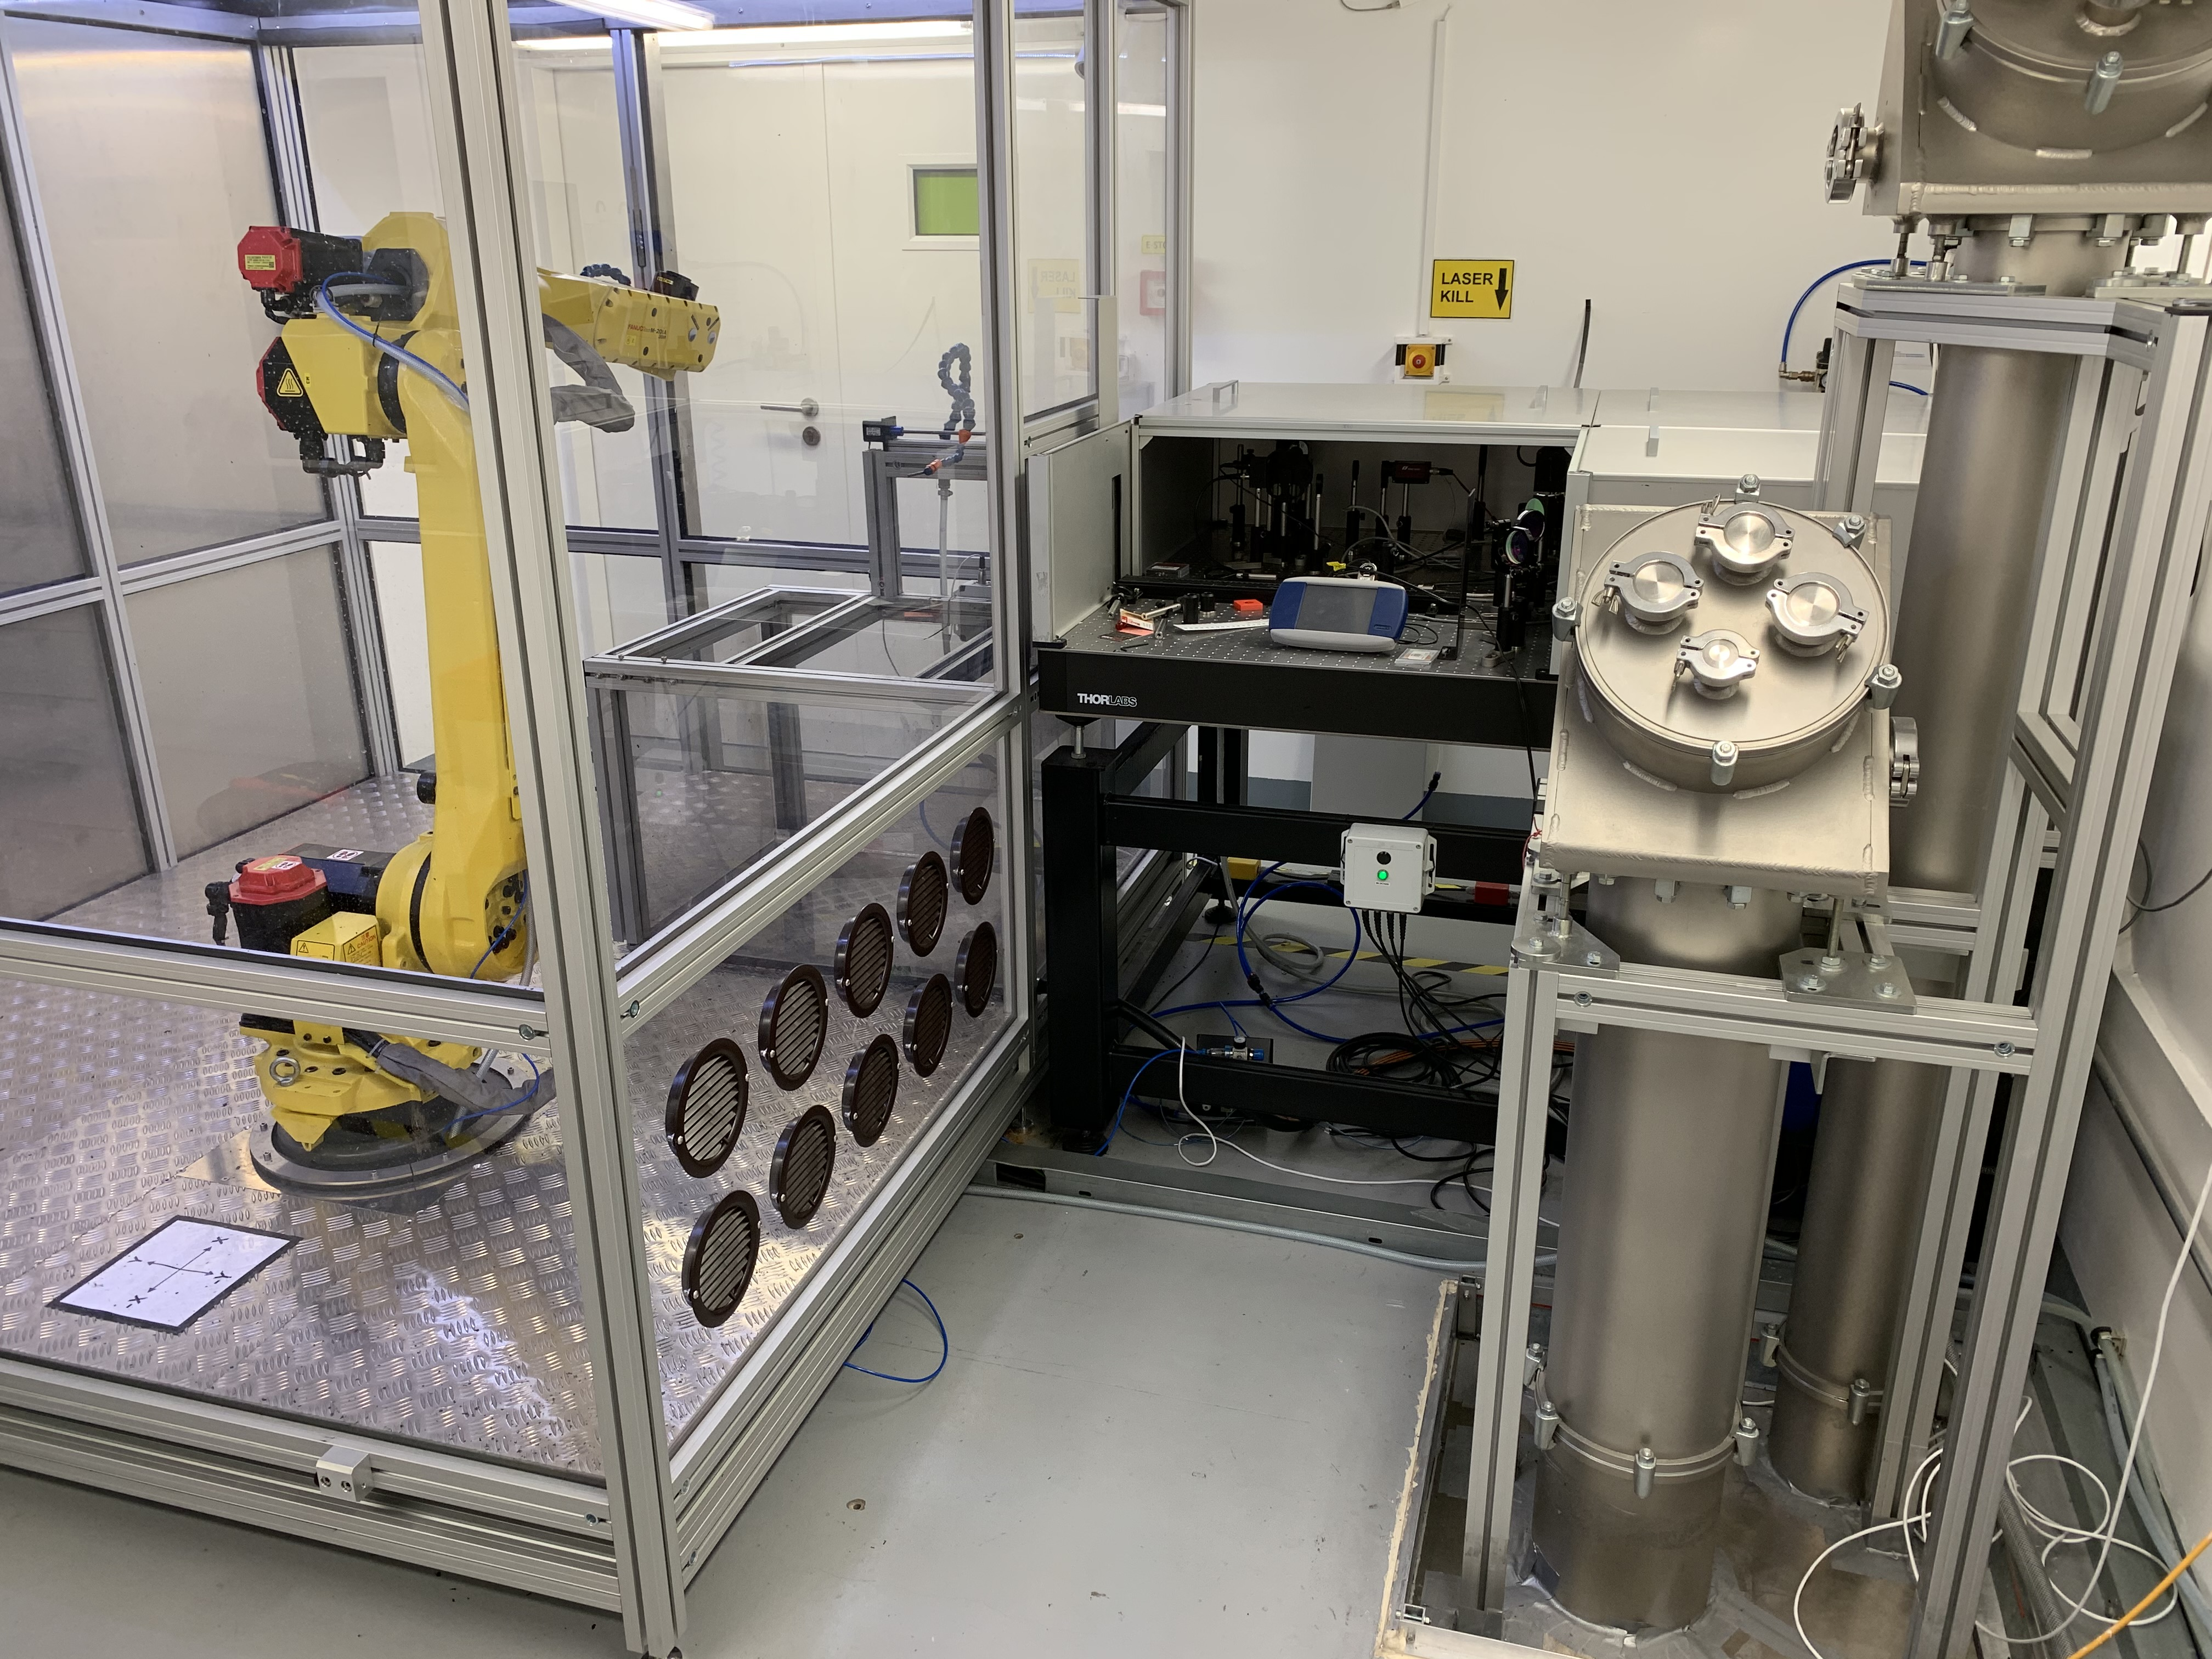
\includegraphics[width=1\linewidth]{img/lsp_station_real.JPG}

    \label{fig:b}
\end{subfigure}

\caption{(Description of images from left to right) (1) schematic layout of LSP station, (2) photography of LSP station \cite{bohm_kaufman_brajer_rostohar_2019}}
\label{fig:lsplayout}
\end{figure}



\subsection{Bivoj laser system}

\subsubsection*{Bivoj front-end}

The front-end starts with a fibre-based section, consisting
of a fibre oscillator, a fibre amplifier, and a temporal pulse shaper
with \SI{125}{\ps} resolution. The output of the fibre front-end is fed
to the first booster amplifier, which is regenerative and
increases the energy to \SI{30}{\milli\joule} and reduces the repetition rate to \SI{10}{\hertz}. The second booster amplifier works in a multi-pass regime
and increases the pulse energy to approximately \SI{30}{\milli\joule}.
The repetition rate can be switched between \SI{1}{\hertz} and \SI{10}{\hertz}. The
beam shape at the front-end output is \SI{8 x 8}{\mm\squared} square flat top.

\subsubsection*{Bivoj 10 J amplifier}

The \SI{10}{\joule}  amplifier is the first-stage main amplifier based on
cryogenically cooled multislab technology. The principal
component of the amplifier is the amplifier head, where the
gain media are stored and cooled by gaseous helium to 
the temperature of about \SI{150}{\kelvin}. The laser beam from the front-end
is enlarged to \SI{22 x 22}{\mm\squared} and sent to the \SI{10}{\joule} amplifier, where
increases its pulse energy from approximately \SI{30}{\milli\joule} to
approximately \SI{8}{\joule} at \SI{10}{\hertz}. The spatial profile of the laser beam at the output of the Bivoj \SI{10}{\joule} amplifier is shown in Figure \ref{fig:spatialprofile} and the temporal profile is shown in Figure \ref{fig:temporalprofile} \cite{saumyabrata}.

\begin{figure}[h]
    \centering
    \includegraphics[width=0.6\linewidth]{img/spatial_profile.jpg}
    \caption{Spatial profile of laser beam at output of Bivoj \SI{10}{\joule} amplifier and approximate dimensions \cite{kaufman}}
    \label{fig:spatialprofile}
\end{figure}

\begin{figure}[h]
    \centering
    \includegraphics[width=0.6\linewidth]{img/bivoj_temp.png}
    \caption{Temporal profile of laser beam at output of Bivoj \SI{10}{\joule} \cite{kaufman}}
    \label{fig:temporalprofile}
\end{figure}

\subsection{Litron LPY ST 7875-10 2HG laser}

The second laser source available at the LSP station is the Litron LPY ST 7875-10 2HG laser, a tabletop laser located directly in the experimental laboratory next to the LSP station. This laser is a pulsed Q-switched Nd:YAG laser suited for industrial or research applications. The Litron  LPY ST 7875-10 2HG laser comes with a super-gaussian resonator. The most important parameters of this system are highlighted in Table \ref{tab:litronparameters} and the laser system is shown in Figure \ref{fig:litron} \cite{litron}. 


\begin{table}[h!] 
\centering
    \begin{threeparttable}
        \begin{tabular}{|c | c|} 
        \hline
            \textbf{Parameter} & \textbf{Value} \\ [0.5ex] 
        \hline
        Repetition Rate [Hz] & 10  \\ 
        \hline
            Output Energy [mJ] & \\
            1064nm & 3500 \\
            532nm & 1750 \\
        \hline
            Beam Diameter [mm] & 15 \tnote{a} \\
        \hline
            Beam Divergence [mrad] & <0.5 \tnote{b} \\ 
        \hline
            Pulse Length @1064nm [ns] & 10-12 \\
        \hline
            Pointing Stability [µrad] & 25 \tnote{c} \\
        \hline
            Timing Jitter [ns] & <0.5 \tnote{d}  \\
        \hline
        \end{tabular}
        \begin{tablenotes}
            \small
            \item[a] Peak-to-peak Energy -- 99 \% of pulses. 
            \item[b] Full angle for 90 \% of the energy.
            \item[c] Half angle.
            \item[d] Jitter is measured concerning the external Q-switch trigger input.
        \end{tablenotes}
        
    \end{threeparttable}
        \caption{Litron LPY ST 7875-10 2HG parameters \cite{litronmanual}}
\label{tab:litronparameters}
\end{table}

\begin{figure}[h]
    \centering
    \includegraphics[width=0.6\linewidth]{img/litron.JPG}
    \caption{Litron LPY ST 7875-10 2HG laser at HiLASE centre}
    \label{fig:litron}
\end{figure}





\subsection{FANUC M-20iA/20M robotic arm}

The FANUC M-20iA/20M is a 6-axis universal industrial robotic arm with a maximum load capacity of \SI{20}{\kg} and a maximum reach of \SI{1811}{\mm}. The repeatability of the robotic arm is \SI{+-0.08}{\mm}. The FANUC M-20iA/20M is a multipurpose robotic arm and can be used for various applications such as assembling, packaging and machining \cite{fanucrobot}.

The robotic arm is coupled with a FANUC R-30iB controller. The R-30iB controller is equipped with a FANUC AIF01A PLC interface module. The interface module is connected to the following expansion modules:

\begin{itemize}
    \item AID16L -- 16 digital inputs,
    \item AOD16D -- 16 digital outputs,
    \item ADA02A -- 2 analog outputs. \cite{fanucunitmanual}
\end{itemize}

The FANUC AIF01A PLC interface module and its expansion modules are connected to the Bivoj and Litron lasers via digital inputs and outputs. In the case of the Bivoj laser system, the expansion modules are linked to a fast flipper located in the Bivoj laboratory. The fast flipper either redirects the laser beam into a cooled beam dump or lets it pass through the LBDS into the LSP station. The Litron laser is coupled to the robotic arm controller via an external trigger. 

\subsection{Electrical connection between FANUC R-30iB controller and Litron LPY ST 7875-10 2HG laser}

A block diagram of the electrical connection between FANUC R-30iB controller and Litron LPY ST 7875-10 2HG laser is shown in Figure \ref{fig:electronics}. The robotic arm PLC sends out a \textit{ROBOT GATE} digital output signal which acts as a gating signal for the \textit{EXTERNAL TRIGGER INPUT} signal. The \textit{EXTERNAL TRIGGER INPUT} signal is generated by the microcontroller unit (MCU). The \textit{LAMP SYNC OUTPUT} signal is fed back to the MCU and to the delay generator. The delay generator creates a delayed \textit{Q-SWITCH TRIGGER} signal which is inputed into the D/A  input of the laser controller. The \textit{Q-SWITCH TRIGGER} signal is delayed with respect to the \textit{LAMP SYNC OUTPUT} signal by $t_{QSW}$. The value of $t_{QSW}$ is fine-tuned with the help of the delay generator.  The timing diagram for internal triggering of the flashlamps and external triggering of the q-switch is shown in Figure \ref{fig:wave}, where:

\begin{itemize}
    \item $t_{BT}$ -- intra-cavity build up time (typically \SIrange{50}{100}{\ns}),
    \item $t_{QSW}$ -- timed by external electronics with respect to external lamp trigger input (typically \SIrange{100}{500}{\us} for maximum output)

\end{itemize}


\begin{figure}[h]
    \centering
    \includegraphics[width=1.0\linewidth]{img/electronics_3.jpg}
    \caption{Block diagram of the electrical connection between FANUC R-30iB controller and Litron LPY ST 7875-10 2HG laser}
    \label{fig:electronics}
\end{figure}

\begin{figure}[h]
    \centering
    \includegraphics[width=1.0\linewidth]{img/wavedrom_bigger.png}
    \caption{Timing diagram for external triggering of flashlamp and internal triggering of the q-switch, where $t_{BT}$ is the intra-cavity build up time (typically \SIrange{50}{100}{\ns}) and $t_{QSW}$ is the internally timed q-switch delay (typically \SIrange{100}{500}{\us} for maximum output)}
    \label{fig:wave}
\end{figure}


The  FANUC M-20iA/20M robot and FANUC R-30iB controller are shown in Figure~ \ref{fig:robotcontroller} \cite{fanucrobotcontroller}. The electrical connection also allows to change the repetition rate of the laser (1 \SI{}{\hertz} or 10 \SI{}{\hertz}).


\begin{figure}[h]
\centering
\begin{subfigure}{.45\textwidth}

    \includegraphics[width=1\linewidth]{img/fanuc_robot.png}

    \label{fig:a}
\end{subfigure}
\begin{subfigure}{.45\textwidth}

    \includegraphics[width=1\linewidth]{img/fanuc_controller.png}

    \label{fig:b}
\end{subfigure}

\caption{(Description of images from left to right) (1) FANUC M-20iA/20M industrial robotic arm, (2) FANUC R-30iB controller with Teach Pendant \cite{fanucrobotcontroller}}
\label{fig:robotcontroller}
\end{figure}



\begin{comment}
\begin{figure}[h]
    \centering
    \includegraphics[width=0.6\linewidth]{img/fanuc_robot.png}
    \caption{FANUC M-20iA/20M industrial robotic arm  \cite{fanucrobot}.}
    \label{fig:fanucrobot}
\end{figure}
\end{comment}

\subsection{Network connection of robot controller}


The robot controller must be reachable from the computer running the RoboDK application described in \hyperref[chap:design]{Chapter 3 -- Design}. In the LSP station this is ensured by having the controllers and computer on the same local network as depicted in Figure \ref{fig:network}. 

\begin{figure}[h]
    \centering
    \includegraphics[width=0.8\linewidth]{img/network.pdf}
    \caption{Network diagram of the robotic arm workcell}
    \label{fig:network}
\end{figure}


\subsection{LSP process example}

The following \href{https://www.youtube.com/watch?v=awhlLU91-dk&ab_channel=HiLASECentre}{video} shows the improvement of cavitation erosion resistance by LSP carried out at the HiLASE centre. This process is developed by HiLASE center and SIGMA GROUP Plc. for the improvement of cavitation erosion resistance of pump blades. The parameters chosen for this experiment are shown in Table \ref{experimentalparameters}. 

\begin{table}[h!]
\centering
    \begin{threeparttable}
        \begin{tabular}{|c | c|} 
        \hline
            \textbf{Parameter} & \textbf{Value} \\ [0.5ex] 
        \hline
        Laser source & Bivoj laser system  \\
        \hline
        Wavelength [\SI{}{\nano\second}] & 1030 \\
        \hline
        Repetition Rate [\SI{}{\hertz}] & 10  \\ 
        \hline
            Pulse energy at sample [\SI{}{\milli\joule}] & 5000 \\
        \hline
            Beam size at sample [\SI{}{\mm\squared}] & 4 \\
        \hline
            Pulse Length @1030nm [\SI{}{\nano\second}] & 10 \\
        \hline
            Beam size at sample [\SI{}{\giga\watt\per\cm\squared}] & 5.56 \\

        \hline
        \end{tabular}

        \caption{Experimental parameters of laser shock peening for improvement of cavitation erosion resistance}
        \label{experimentalparameters}
    \end{threeparttable}
\end{table}



\chapter{Design}

    \epigraph{If you drive a car, it makes little difference what brand it is: all cars are driven
in essentially the same way. The same applies to computers. If you have a
Windows PC, the user interface won’t be affected by your computer hardware.
This is definitely not the case for industrial robots.}{\textit{Albert Nubiola \\ CEO at RoboDK}}

This chapter gets the reader acquainted with the RoboDK software and its various features. This is followed by  \autoref{chap:implementation}, where this knowledge will be used practically. 

\section{RoboDK overview}

RoboDK (short for robot development kit) is a development platform for industrial robotic arm offline programming and simulation. 

\subsection{RoboDK history}

RoboDK (the company) was founded by Albert Nubiola and Lauren Ierullo in January 2015 as a spin-off company from the \href{https://en.etsmtl.ca/unites-de-recherche/coro/accueil?lang=en-CA}{CoRo laboratory}   at ETS University in Montreal, Canada. RoboDK is a commercial version of \href{https://www.parallemic.org/RoKiSim.html}{RoKiSim}, a multiplatform educational software tool for 3D simulation of serial 6-axis robotic arms.

\subsection{RoboDK features}


The following section highlights some of the features RoboDK has to offer: 


\begin{itemize}
\item graphical user interface,
\item drag-and-drop functionality, 
\item support for 3D file formats - importing objects and creating new tools using 3D files such as \mintinline{shell-session}{STL}, \mintinline{shell-session}{STEP} and \mintinline{shell-session}{IGES},
\item CAD-to-path features - generating robot programs directly from curves placed on station objects 
\item external axes - integrating external axes to extend the robotic arm’s reachability,
\item generating programs - generating programs for various robotic arm manufacturers,
\item running programs on the fly – executing programs directly from an external computer,
\item real-time monitoring – viewing the robotic arm state on an external computer,
\item computer aided manufacturing for robotic arms - converting 5-axis CNC toolpaths to robotic arm programs and using a robotic arm like a 5-axis CNC,
\item automated path solving - avoiding robotic arm errors, including singularities, joint limits and collisions,
\item fast collision detection - defining the object interactions, 
\item advanced use - creating robotic arm programs from an external computer using a higher programming language. The RoboDK API is available in Python, C\#, Visual Basic, C++, and Matlab,
\item simulating 2D vision cameras - testing image recognition algorithms in the simulation environment,
\item multiple robotic arms simulation - synchronizing and programming multiple robotic arms and moving them at the same time, 
\item customizable post processors - integrating specific sensors or actuators such as grippers, force control, image processing, etc.
\end{itemize}

\subsection{RoboDK licence and versions}

RoboDK offers free (limited), educational or professional versions. 
The software is available for Windows, MacOS, Ubuntu Linux, Android or iOS. It supports either 32-bit or 64-bit versions of the abovementioned operating systems. At the time of writing this document, the latest version of RoboDK is 5.2. The complete RoboDK revision history is available \href{https://robodk.com/whatsnew}{online}. 

\section{RoboDK robot library}

RoboDK supports offline programming and has an extensive robotic arm library supporting robotic arm controllers from various manufacturers, including, but not limited to:

\begin{itemize}
    \item ABB 
    \item Fanuc 
    \item KUKA 
    \item Motoman 
    \item Universal Robots 
\end{itemize}
Models of industrial robotic arms in RoboDK have the same properties as if used with an actual robotic arm controller. The RoboDK library can be accessed \href{https://robodk.com/library}{online} either via a browser or in the RoboDK application itself (keyboard shortcut - \mintinline{shell-session}{Ctrl+Shift+O}).


\section{RoboDK interface}

The interface of RoboDK consists of the main menu, the toolbar, the station tree, the status bar, and the 3D view. A picture of the RoboDK interface is shown in Figure \ref{fig:robodkinterface}. An extensive documentation for RoboDK is available \href{https://robodk.com/doc/en/Basic-Guide.html#Start}{online}.

\subsection{RoboDK station}

A RoboDK project containing a robotic arm, robotic arm tools, additional CAD files, robotic arm frames, and a robotic arm program is called a station. A RoboDK station is saved as one file (\mintinline{shell-session}{.rdk} extension).  The FANUC M-20iA/35M model from the RoboDK robotic arm library is used in this thesis because it is readily available in the RoboDK library and differs from the FANUC M-20iA/20M robotic arm used in the LSP station at HiLASE only in payload capacity. Robot files in RoboDK have a \mintinline{shell-session}{.robot} extension.

\begin{figure}[h]
    \centering
    \includegraphics[width=0.9\linewidth]{img/robodk_interface.png}
    \caption{RoboDK interface v 5.2 running on Windows 10.}
    \label{fig:robodkinterface}
\end{figure}

\section{RoboDK API}

RoboDK provides a graphical user interface (GUI) to simulate and program industrial robotic arms. No programming experience is required to simulate and program robotic arms using the GUI. Unfortunately, the GUI has some limitations when used for simulation and offline programming. If such a situation arises, then the RoboDK application interface (API) can be used to extend the capabilities of RoboDK.

The API exposes a set of routines and commands to RoboDK, enabling the user to program the robotic arm using high-level programming languages. The RoboDK API is available for Python, C\#, C++, Visual Basic (.NET) and Matlab. Any of these programming languages can be used to simulate and program any robotic arm. The API can conveniently handle the following tasks:

\begin{itemize}
    \item Automating simulation
    \item Offline programming
\end{itemize}

The RoboDK API is divided into the following modules:


\begin{itemize}
    \item \mintinline{shell-session}{robolink} module - this module represents the link between RoboDK and the high-level programming language,
    \item \mintinline{shell-session}{item} module - any item from the RoboDK item tree can be retrieved.  An item can be a robotic arm, a reference frame, a tool, an object, or a specific project,
    \item \mintinline{shell-session}{robodk} module - a module with a robotics toolbox for pose operations. All post processors depend on the \mintinline{shell-session}{robodk} module.
\end{itemize}

\section{RoboDK Add-ins}

\subsection{RoboDK Add-in interface}

Add-ins extend RoboDK's functionality. Add-ins can be developed by using the RoboDK Add-in interface. The RoboDK Add-in interface is linked natively to the core of RoboDK.

\subsection{RoboDK Add-in for SolidWorks}

Solidworks is a professional 3D CAD modelling application. The RoboDK Add-in for SolidWorks allows to combine SolidWorks 3D CAD modelling features with robotic arm simulation and offline programming in RoboDK and considerably simplifies the programmer's workflow. The programmer can load the 3D models created in SolidWorks directly to RoboDK. Groups of curves or points can also be loaded to RoboDK, and robotic arm programs can be generated from the curves or points subsequently.

\subsubsection*{SolidWorks RoboDK Add-in toolbar}

The RoboDK Add-in for SolidWorks is accessible directly from the SolidWorks toolbar.  The RoboDK Add-in in SolidWorks is shown in Figure  \ref{fig:solidworkstoolbar}. The Add-in toolbar presents the programmer with several functionalities:

\begin{itemize}
    \item \mintinline{shell-session}{AutoSetup} - the user selects the geometry (curves and points) and the model, the curves are automatically transferred to RoboDK,
    \item \mintinline{shell-session}{LoadPart} - only loads the 3D model from SolidWorks to RoboDK without importing the curves or points,
    \item \mintinline{shell-session}{LoadPoints} - loads points to RoboDK as a new object. Selected surfaces are used to calculate the curve normals, 
    \item \mintinline{shell-session}{Load Curves} -  loads curves selected in RoboDK as a new object. Selected surfaces are used to calculate curve normals, 
    \item \mintinline{shell-session}{Settings} - opens default settings window.
\end{itemize}

\begin{figure}[h]
    \centering
    \includegraphics[width=0.6\linewidth]{img/solidworks_toolbar.PNG}
    \caption{SolidWorks RoboDK Add-in Toolbar.}
    \label{fig:solidworkstoolbar}
\end{figure}


%%%%%% TO MUCH USELESS INFORMATION, WILL BE LEFT OUT FOR NOW %%%% 

\begin{comment}

\subsubsection*{Importing curves from Solidworks}

To import curves from SolidWorks to RoboDK, SolidWorks offers two options:

\begin{enumerate}

\item PŘEDĚLAT FORMU, ABY BYLO PODOBNÉ.

\item \textbf{Opening an existing RoboDK station} - Using the \mintinline{shell-session}{Settings} control element of the SolidWorks RoboDK Add-in and then selecting the current project with the \mintinline{shell-session}{Load Project...} button. The next step is to click the \mintinline{shell-session}{LoadCurves} button and highlight the curves that define the robotic arm path and the adjacent surfaces of these curves. Lastly, the action is confirmed by pressing the \mintinline{shell-session}{checkmark} button. The curve is then opened in the selected project. 

\item \textbf{Creating a new RoboDK station} - In this case, the robot path is selected the same way as described in the previous point. A new RoboDK station containing the robotic arm path is opened after pressing the \mintinline{shell-session}{checkmark} button.

\end{enumerate}

\end{comment}


\section{RoboDK post processors}

Post processors generate robot programs for robot controllers from robot simulations. Post processors are essential for offline programming of robots. A post processor defines the vendor-specific rules a robot program must follow. A robotic arm must be linked to a post processor in RoboDK to be able to generate a robotic arm controller program. The post processors available in RoboDK by default can be found \href{https://robodk.com/doc/en/Post-Processors.html#AvailablePosts}{online}.  
A post processor in RoboDK is a Python script (\mintinline{shell-session}{.py} extension). All the post processors of RoboDK are located in the
\mintinline{shell-session}{C:/RoboDK/Posts/} folder (in case of the Windows operating system).  To use a post processor it must be placed in the \mintinline{shell-session}{C:/RoboDK/Posts/} folder. The user can modify an existing post processor or create a new one from scratch. Modifications of post processors are described in \autoref{chap:implementation} in more detail. 

\chapter{Implementation}

    \label{chap:implementation}

\epigraph{Python is the "most powerful language you can still read".}{\textit{Paul Dubois \\ Lead developer for Numerical Python and Pyfort }}

This chapter deals with creating a curve follow project in RoboDK and modifying a RoboDK post processor to be suitable for the LSP process.

\section{FANUC robotic arms programming specifics and FANUC software}

\subsection{FANUC Roboguide}

FANUC Roboguide is a proprietary robot simulator and offline programming tool developed by FANUC. Roboguide is in many ways similar to RoboDK.  Like RoboDK, it supports the creation of robotic arm stations, importing of CAD files and CAD--to--path features. The main difference is that Roboguide is limited to FANUC robotic arms and FANUC related technologies and procedures. In contrast, RoboDK is not limited to one robotic arm manufacturer and is universal and expandable. Roboguide is used for this project to compile the created FANUC programs and upload them to the FANUC robotic arm controller. Roboguide offers several simulation software options tailored for specific robotic arm applications:

\begin{itemize}

\item FANUC Roboguide HandlingPRO -- simulating material handling applications including load/unload, packaging, assembly and material removal,
\item FANUC Roboguide PaintPRO -- simulating painting applications,
\item FANUC Roboguide WeldPRO -- simulating robotic arc welding processes,
\item FANUC Roboguide PalletPRO and PalletTool -- simulating palletizing applications.

\end{itemize}

An example of a Roboguide station is shown in Figure \ref{fig:roboguide}. The version of FANUC Roboguide used for this project is 8.30104.00.35 (Rev. K) \cite{roboguide}. 

\begin{figure}[h]
    \centering
    \includegraphics[width=0.9\linewidth]{img/roboguide.PNG}
    \caption{FANUC Roboguide workcell -- user interface example}
    \label{fig:roboguide}
\end{figure}

\subsection{FANUC robotic arm controller programming languages}

The FANUC company implements two programming languages for programming their robot controllers: teach pendant (TP) or KAREL. The TP language is mainly used for motion control of the robotic arm and the programs are usually edited via the pendant. TP programs are either binary files (\mintinline{shell-session}{.tp} file extension) or can be human--readable ASCII files (\mintinline{shell-session}{.ls} file extension). The KAREL language is a high--level language and does not support robotic arm movement instructions. KAREL is mainly used to implement program logic. KAREL programs can not be edited using a pendant.

\subsection{Compiling a FANUC TP program}

Only a TP program in binary format can be run on FANUC robotic arm controllers. Because RoboDK creates TP programs as human--readable ASCII files, the TP programs need to be converted to binary format before uploading them to the robot controller. Two options to convert \mintinline{shell-session}{.ls} programs to \mintinline{shell-session}{.tp} programs exist:

\begin{enumerate}
\item the ASCII Upload option must be loaded on the robot controller. After upload an \mintinline{shell-session}{.ls} file to the controller it is automatically converted to a \mintinline{shell-session}{.tp} file,
\item the program is compiled and uploaded either using the WinOLPC  tools via Roboguide or using the WinOLPC tools directly \cite{fanuchandling}.

\end{enumerate}

\section{Robot machining projects in RoboDK}

The applications of robot machining in the industry are numerous. Some applications include:

\begin{itemize}

    \item milling,
    \item drilling,
    \item chamfering,
    \item deburring.

\end{itemize}

RoboDK offers three types of robot manufacturing projects:

\begin{itemize}

    \item robot machining projects,
    \item curve follow projects, 
    \item point follow projects. 

\end{itemize}

The process of setting up a curve follow project in RoboDK is described in the following sections. In laser shock peening, the laser (representing the tool) is static, and the robot holds the object. Therefore, a curve follow project with a constant tool orientation is set up in RoboDK \cite{machiningproject}.

\subsection{Setting up a curve follow project in RoboDK}

A curve follow project in RoboDK must at least consist of one robot, one tool, and one reference frame. The situation described is a so--called remote TCP situation, i.e., the Tool Center Point (TCP) is fixed in the station, and the robot holds the object. The TCP in our project is represented by the laser beam. 
The user has to execute the following steps to set up a basic curve follow project: 

\begin{enumerate}

\item create and import the robotic arm path to RoboDK using preferred CAD software,

\item mount the robot path as a tool in RoboDK,

\item import the robotic arm and create reference frame (optionally import CAD of manufactured part) into RoboDK station, 

\item create curve follow project: \mintinline{shell-session}{Utilities} $\rightarrow$ \mintinline{shell-session}{Curve follow project},

\item open the curve follow project settings. A window similar to the one displayed in Figure \ref{fig:curvefollow} will open, 

\item modify curve follow project settings:

    \begin{itemize}

        \item \mintinline{shell-session}{Robot}: the robotic arm holding the object,
        \item \mintinline{shell-session}{Reference}: the frame representing the remote TCP,
        \item \mintinline{shell-session}{Tool}: the robotic arm path.
        
    \end{itemize}
    
\item change \mintinline{shell-session}{Select algorithm} option to: \mintinline{shell-session}{Robot holds object & follows path},

\item update project. RoboDK automatically generates a preprocessed robot program for the actual station,

\item right--click the preprocessed program, select post processor and generate program. The \mintinline{shell-session}{.ls} program for the actual station will be opened in the default RoboDK text editor,

\item compile the program and export the program to the FANUC robot controller using Roboguide or WinOLPC tools \cite{curvefollow}.
    
\end{enumerate}

\begin{figure}[h]
    \centering
    \includegraphics[width=0.9\linewidth]{img/curve_follow_settings.PNG}
    \caption{Curve follow project settings in RoboDK}
    \label{fig:curvefollow}
\end{figure}

\section{RoboDK API}

An application interface is a set of features an application provides to a user via a high--level programming language. The RoboDK API dramatically expands the possibilities of RoboDK. The RoboDK API is implemented in The RoboDK API is implemented in Python, C\#, C++, Visual Basic (.NET) and Matlab.  The Python API is the most extensive and is used in this thesis. The RoboDK API facilitates the execution of the following tasks:

\begin{itemize}
    
 \item Automating simulation -- macro scripts for repetitive tasks such as tool changing, pick and place applications.

 \item Offline programming -- using the RoboDK API methods to create programs for specific robotic arm controllers. The pre--processed \mintinline{shell-session}{.pyc} file created in RoboDK's GUI is executed directly by the post processor. The post processor defines the rules for vendor--specific robotic arm controller program generation. 

 \item Online programming -- using RoboDK API to move robots and retrieve their current position in real time. RoboDK connects to the robotic arm controller using robot drivers.

\end{itemize}

The elegance of this approach is that the same program written in a high--level programming language can be used for all three of the abovementioned tasks \cite{robodkapi}. 

\subsection{Python API for RoboDK}

Python is an interpreted high--level programming language. The Python API for RoboDK uses Python 3, although most features are compatible with Python 2 also. The RoboDK API for Python consists of the following modules:

\begin{itemize}
    \item \mintinline{text}{robolink} module -- this module represents the link between RoboDK and the high--level programming language,
    \item \mintinline{text}{item} module -- any item from the RoboDK item tree can be retrieved.  An item can be a robotic arm, a reference frame, a tool, an object, or a specific project,
    \item \mintinline{text}{robodk} module -- a module with a robotics toolbox for pose operations. All post processors depend on the \mintinline{text}{robodk} module .
\end{itemize}

The modules are located in the folder \mintinline{shell-session}{C:/RoboDK/Python/} in the Windows operating system. This folder is included in the \mintinline{shell-session}{PYTHONPATH} system variable. The Python API is accompanied with examples. These examples are located in the folders \mintinline{shell-session}{C:/RoboDK/Library/Scripts}  and \mintinline{shell-session}{C:/RoboDK/Library/Macros}  in the Windows operating system \cite{robodkapipython}.

\section{RoboDK post processors}

A post processor specifies how robot programs must be generated for a specific robot controller and are used when robotic arm controllers are generated offline. Post processors serve as tools to convert the simulation to vendor--specific robot programs. All RoboDK post processors are placed in the \mintinline{shell-session}{C:/RoboDK/Posts} folder in the Windows operating system. All post processors rely on the \mintinline{shell-session}{robodk} module. The \mintinline{shell-session}{robodk} module is a robotics toolbox for Python, based on \href{http://petercorke.com/Robotics_Toolbox.html}{Peter Corke’s Robotics Toolbox} \cite{robodkapipython}. 

\subsection{RoboDK preprocessed file}

After creating a program in the curve follow project, but before generating it using a post processor, the program is saved as a preprocessed/universal Python program and saved in a local temporary folder. The preprocessed program is linked to the right post processor (selected by the user in RoboDK). The post processor defines a \mintinline{python}{RobotPost} class that generates the desired code. In the Windows operating system, the preprocessed Python files are saved in the user's temporary folder (e.g.: \mintinline{shell-session}{C:/Users/username/AppData/Local/Temp}) folder. These programs can also be used for debugging new post processors. An example code of a preprocessed file is shown in Listing \ref{code:preprocessed_python} \cite{preprocessed}:

%% this is an example of a minted code with caption and wrapped lines

\label{code:preprocessed_python}
\begin{minted}[frame=lines, linenos,tabsize=2,breaklines]{python}
import sys
import os
sys.path.append(os.path.abspath(r"""C:/RoboDK/Posts/""")) # temporarily add path to POSTS folder

from FANUC_R30iA_decompyle3 import *

def p(x,y,z,r,p,w):
  a = r*math.pi/180.0
  b = p*math.pi/180.0
  c = w*math.pi/180.0
  ca = math.cos(a)
  sa = math.sin(a)
  cb = math.cos(b)
  sb = math.sin(b)
  cc = math.cos(c)
  sc = math.sin(c)
  return Mat([[cb*ca,ca*sc*sb--cc*sa,sc*sa+cc*ca*sb,x], [cb*sa,cc*ca+sc*sb*sa,cc*sb*sa--ca*sc,y], [--sb,cb*sc,cc*cb,z], [0.0,0.0,0.0,1.0]])

print('Total instructions: 140')
r = RobotPost(r"""FANUC_R30iA_decompyle3""",r"""Fanuc M--20iA/35M""",6, axes_type=['R','R','R','R','R','R'], ip_com=r"""127.0.0.1""", api_port=20500, prog_ptr=2172227036784, robot_ptr=2172252511552)

r.ProgStart(r"""Settings""")
r.RunMessage(r"""Program generated by RoboDK v5.2.2 for Fanuc M--20iA/35M on 02/07/2021 17:12:29""",True)
r.RunMessage(r"""Using nominal kinematics.""",True)
r.setZoneData(1.000)
r.setSpeed(1000.000)
r.setFrame(p(1000.3,--445,552.3,0,10.19,--90),--1,r"""LASER_RTCP""")
r.setTool(p(0,0,0,0,0,0),--1,r"""ZAPUSTKA_PATH""")
r.RunMessage(r"""Show ZAPUSTKA_PATH""",True)
r.MoveJ(None,[--9.2878,0.949114,--28.3094,94.4347,--81.8311,87.4811],None)
r.MoveL(p(--14.8303,41.4662,85,105.917,0,180), [--14.8823,2.45519,--28.2667,97.1731,--76.9261,87.0176], [0,0,0])
r.setSpeed(10.000)
r.MoveL(p(0.866853,42.1343,85,94.455,0,180), [--14.6627,3.59506,--28.447,97.1044,--77.1403,75.3963], [0,0,0])
r.MoveL(p(11.9961,40.7679,85,85.5416,0,--180), [--14.5062,4.37964,--28.4381,97.0241,--77.2757,66.5094], [0,0,0])
r.MoveL(p(16.6541,40.7679,85,85.5416,0,180), [--14.4431,4.71382,--28.4699,96.9996,--77.3347,66.484], [0,0,0])

...
...
...

r.MoveL(p(--16.8929,40.7854,85,108.509,0,180), [--14.9101,2.29849,--28.2014,97.1719,--76.8936,449.673], [0,0,0])
r.setSpeed(1000.000)
r.MoveL(p(--16.1785,41.074,185,107.509,0,180), [--9.29955,0.844572,--28.2678,94.4344,--81.8176,449.114], [0,0,0])
r.ProgFinish(r"""Settings""")
r.ProgSave(r"""C:/Users/marek.boehm/Documents/RoboDK/""", r"""Settings""", False, r"""C:/RoboDK/Other/VSCodium/VSCodium.exe""")

\end{minted}
\captionof{listing}{Code snippet of preprocessed program to be executed by post processor}


Let us dive into the source code of this preprocessed file and explain the functionality of some of its methods. The \mintinline{python}{p(x,y,z,r,p,w)} function converts the XYZRPW representation to a Pose ($ 4 \times 4 $ matrix). The \mintinline{python}{RobotPost} class initializes the robot post processor object. The parameters of the \mintinline{python}{RobotPost} class are:

\begin{minted}[frame=lines,tabsize=2,breaklines]{python}

class samplepost.RobotPost(robotpost=None, robotname=None, robot_axes=6, **kwargs)

\end{minted}


Parameters of \mintinline{text}{RobotPost} class:

\begin{itemize}

\item \mintinline{python}{robotpost (string)} -- name of the post processor linked to the preprocessed file,

%% do not highlight anything - then use text
\item \mintinline{text}{robotname(string)} -- the name of the robotic arm,

\item \mintinline{text}{robotaxes(string list)} -- type and quantity of robotic arm axes,

\item \mintinline{text}{**kwargs} -- pass additional arguments to function.

\end{itemize}

All subsequent functions are called upon the \mintinline{python}{RobotPost} object. The most important function is the \mintinline{python}{MoveL} function:


\begin{minted}[frame=lines,tabsize=2,breaklines]{python}

MoveL(pose, joints, conf_RLF=None)

\end{minted}


Parameters \mintinline{text}{MoveL} method:

\begin{itemize}

\item \mintinline{text}{pose (robodk.Mat())} -- pose target of the tool with respect to the reference frame, pose can be \mintinline{python}{None} if the target is defined as a joint target,

%% do not highlight anything - then use text
\item \mintinline{text}{joints (float list)} -- robot joints as a list,

\item \mintinline{text}{robotaxes(array)} -- type and quantity of robotic arm axes,

\item \mintinline{text}{conf_RLF (int list)} -- pass additional arguments to function. 

\end{itemize}

Another important method in the preprocessed file is the \mintinline{python}{ProgSave} method, which saves the program after all instructions have been executed:


\begin{minted}[frame=lines,tabsize=2,breaklines]{python}

ProgSave(folder, progname, ask_user=False, show_result=False)

\end{minted}


Parameters of \mintinline{text}{ProgSave} method:

\begin{itemize}

\item \mintinline{text}{pose (robodk.Mat())} -- pose target of the tool with respect to the reference frame, pose can be \mintinline{python}{None} if the target is defined as a joint target,

%% do not highlight anything - then use text
\item \mintinline{text}{folder (str)} -- folder hint to save the program,

\item \mintinline{text}{progname (str)} -- program name as a hint to save the program,

\item \mintinline{text}{ask_user (bool, str)} -- true if the default settings in RoboDK are set to promt the user to select the folder, 

\item \mintinline{text}{show_result (bool, str)} -- false if the default settings in RoboDK are set to not show the program once it has been saved. Otherwise, a string is provided with the path of the preferred text editor.

\end{itemize}

 Every post processor should implement a set of basic methods to generate programs for robotic arm controllers correctly. These basic  methods used in the preprocessed file can be found in the \href{https://robodk.com/doc/en/PythonAPI/postprocessor.html#post-processor-methods}{online documentation} \cite{postmethods}.


\subsection{Selecting a post processor}

Each robotic arm has a post processor assigned to it by default. The following steps have to be taken to change the post processor of a robotic arm:


\begin{itemize}
    \item opening the robot panel,
    \item selecting \mintinline{shell-session}{Parameters},
    \item selecting post processor from drop--down list \cite{selectpost}.
\end{itemize}

\subsection{Post processor example and example output}

????Here put a link to you github repo, or a snippet????


\subsection{FANUC R--30iA post processor}

The FANUC R--30iB post processor is located in the \mintinline{shell-session}{C:/RoboDK/Posts/vXX folder}. \mintinline{shell-session}{XX} is a two--digit number and denotes the post processor version. The FANUC R--30iA post processor comes in the form of a \mintinline{shell-session}{.pyc} file (compiled bytecode) and needs to be decompiled to a \mintinline{shell-session}{.py} file with the help of a decompiler. The decompyler used in this thesis is   \href{https://github.com/rocky/python--decompile3}{decompyle3} \cite{decompyle3}.

\section{Modifying the FANUC R--30iB post processor methods} 

The user can create a new post processor from scratch or modify an existing post processor. A post processor for a specific robotic arm controller is a single \mintinline{shell-session}{.py} file. All post processors are placed in the \mintinline{shell-session}{C:/RoboDK/Posts} folder. A new post processor is added to RoboDK by creating a \mintinline{shell-session}{.py} file or renaming an existing \mintinline{shell-session}{.py} file in this folder. By deleting a \mintinline{shell-session}{.py} file in this folder, the post processor is deleted from the list of post processors in RoboDK. 

The experimental setup of the LSP station at the HiLASE centre links the robotic arm controller to the laser source. The objective of the post processor modification can be expressed as:

% dirtytalk package

\say{The laser source is operating at a \SI{1}{\hertz} repetition rate. The post processor for the  R--30iB controller will be modified in such a way that when the robotic arm with the sample is in a position, where the LSP process (individual laser impact area) should be placed, the robotic arm controller sends a command to the laser source to fire exactly one laser pulse onto the desired area and then move on to the next position. This is accomplished by controlling the digital inputs (DIs) and digital outputs (DOs) of the robotic arm controller.} 

The modification involves the \mintinline{python}{MoveL} method. The original \mintinline{python}{MoveL} method generates the following code:


\begin{minted}[frame=lines,tabsize=2,breaklines]{text}

L P[2] 4mm/sec CNT100;

\end{minted}


where:

\begin{itemize}

    \item \mintinline{text}{L} -- linear movement,
    \item \mintinline{text}{P[2]} -- designation of point,
    \item \mintinline{text}{4mm/sec} -- movement speed,
    \item \mintinline{text}{CNT100} -- zone data.

\end{itemize}

The modified MoveL method should output the following robotic arm controller code to meet the requirements on the post processor:


\begin{minted}[frame=lines,tabsize=2,breaklines]{text}

WAIT DI[1:SYNCHRONIZATION_IN]=OFF;
WAIT DI[1:SYNCHRONIZATION_IN]=ON;
L P[6] 4mm/sec CNT100 RTCP TB  0.00sec,DO[5]=PULSE,1.0sec;
WAIT  DO[5:LASER ON] = OFF;
WAIT  1.00(sec);
  
\end{minted}


where:

\begin{itemize}

    \item \mintinline{text}{WAIT} -- wait condition,
    \item \mintinline{text}{RTCP} -- remote tool centre point,
    \item \mintinline{text}{TB  0.00sec,DO[5]=PULSE,1.0sec} -- execute command at a designated time before reaching the point,
    \item \mintinline{text}{P[2]} -- designation of point,
    \item \mintinline{text}{DO[5]=PULSE,1.0sec} -- pulse at digital output,
    \item \mintinline{text}{WAIT  1.00(sec)} -- block code execution for a designated time.

\end{itemize}

Listing \ref{code:originalMoveL} contains the original MoveL method of the FANUC R--30iB post processor \cite{postmethods}. 


\label{code:originalMoveL}
\begin{minted}[frame=lines, linenos,tabsize=2,breaklines]{python}

    def MoveL(self, pose, joints, conf_RLF=None):
        """Add a linear movement"""
        if self.LAST_POSE is not None:
            if pose is not None:
                if distance(pose.Pos(), self.LAST_POSE.Pos()) < 0.001:
                    if pose_angle_between(pose, self.LAST_POSE) < 0.001:
                        return
        self.page_size_control()
        if pose is None:
            target_id = self.add_target_joints(pose, joints)
            move_ins = 'P[%i] %s %s ;' % (target_id, self.SPEED, self.CNT_VALUE)
        else:
            target_id = self.add_target_cartesian(pose, joints, conf_RLF)
            move_ins = 'P[%i] %s %s ;' % (target_id, self.SPEED, self.CNT_VALUE)
            # move_ins = 'P[1] %s %s ;' % (self.JOINT_SPEED, self.CNT_VALUE)
        self.addline(move_ins, 'L')
        self.LAST_POSE = pose

\end{minted}
\captionof{listing}{Code snippet of original MoveL method}







\chapter{Testing}

    \label{chap:testing}

Firstly, this chapter deals with the simulation of the LSP process in RoboDK. Secondly, it focuses on testing the robotic arm program on the physical robot. The goal of the testing is to evaluate the effectiveness of the solution in the CAM program RoboDK. The robotic arm cell used for simulation and testing is depicted in section \hyperref[sec:lsp_layout]{\ref{sec:lsp_layout} LSP station layout}. A forging die is used as a test sample. Figure \ref{fig:cad} shows a CAD drawing of the forging die. Figure \ref{fig:cad} also highlights in black the areas to be treated by the LSP process and the approach/retreat motions in green. Information about the areas to be treated by the LSP process is usually provided by the manufacturers based on experience from the factory floor.

\begin{figure}[h]
    \centering
    \includegraphics[width=0.8\linewidth]{img/cad.PNG}
    \caption{CAD drawing of forging die}
    \label{fig:cad}
\end{figure}

\section{Simulation}

The simulation process can be broken down into several steps:

\begin{enumerate}

\item create a robot machining project in RoboDK, so it mirrors the actual robotic arm work cell, 

\item set up the curve follow project, set appropriate collision checking parameters and successfully solve robotic arm path,

\item set appropriate simulation parameters and run simulation,
generate robotic arm program with RoboDK,

\item continue with testing on physical robotic arm.

\end{enumerate}

Figure \ref{fig:robodk_die} shows a picture of the RoboDK work cell with the forging die mounted onto the flange of robotic arm.

\begin{figure}[h]
    \centering
    \includegraphics[width=1.0\linewidth]{img/robodk_cast.PNG}
    \caption{RoboDK work cell with forging die}
    \label{fig:robodk_die}
\end{figure}


\section{Testing on the physical robot}

The testing of robotic arm programs on physical robots follows after the simulation process and is roughly divided into the following steps:

\begin{enumerate}
    
\item upload program to robotic arm controller,

\item run program on physical robotic arm in test mode (test mode = mode of robotic arm with reduced maximum speed) and without laser source,

\item run program on physical robotic arm in production mode (production mode = speed of robotic arm is not restricted),

\item run program in production mode with active laser source. The energy of the laser source is set to a value that is appropriate for the given LSP application. 

\end{enumerate}

Figure \ref{fig:cast} shows the forging die mounted on the robotic arm.

\begin{figure}[h]
    \centering
    \includegraphics[width=1.0\linewidth]{img/cast.jpeg}
    \caption{Forging die mounted on the robotic arm}
    \label{fig:cast}
\end{figure}





\chapter{Discussion}

    \input{chapters/6_discussion}
    
%%%%%%% CONCLUSION CHAPTER %%%%%%%
    
\chapter{Conclusion} % SEM NESAHEJTE!
\addcontentsline{toc}{chapter}{Conclusion} % SEM NESAHEJTE!
%
    Zde napište text úvodu (1-3 strany, nerozdělujte na podkapitoly) nebo jej vložte ze samostatného souboru: např. příkazem \texttt{\textbackslash input\{vnitrek\_zaver.tex\}}.
    
%%%%%%% REFERENCES %%%%%%%

\clearpage  % SEM NESAHEJTE!
\addcontentsline{toc}{chapter}{Reference} % SEM NESAHEJTE!
\printbibliography

\begin{appendices}

    \renewcommand{\chaptermark}[1]{\markboth{#1}{#1}}
    \fancyhead[R]{Appendix \thechapter\ --\ \leftmark}
    \fancyhead[L]{}


    \chapter{Contents of the enclosed CD/DVD}
    \input{appendices/enclosed_cd}

    \chapter{Used software and software libraries}
    \textbf{\LaTeX} - \href{https://miktex.org/}{https://miktex.org/}\newline

\textbf{RoboDK} - \href{https://robodk.com/}{https://robodk.com/}\newline

\textbf{Python} - \href{https://www.python.org/}{https://www.python.org/}\newline

\textbf{decompyle3} - \href{https://github.com/rocky/python-decompile3}{https://github.com/rocky/python-decompile3}\newline

\textbf{SolidWorks Professional 2019} - \href{https://www.solidworks.com/}{https://www.solidworks.com/}\newline

\textbf{RoboDK} - \href{https://robodk.com/}{https://robodk.com/}\newline

\textbf{VSCodium} - \href{https://vscodium.com/}{https://vscodium.com/}\newline

\textbf{Thonny} - \href{https://thonny.org/}{https://thonny.org/}\newline

\textbf{FANUC Roboguide} - \href{https://www.fanucamerica.com/products/robots/robot-simulation-software-FANUC-ROBOGUIDE}{https://www.fanucamerica.com/}\newline


    
    \chapter{Time schedule of thesis}
    \input{appendices/time_schedule}
    
    \chapter{Project budget}
    The following table lists the thesis's operating budget, including purchases of individual components and orders implemented outside school. Prices include VAT and usually including postage and packaging.

\begin{table}[h!]


        \begin{tabular}{|c | c | c | c |} 
        \hline
            \textbf{Component} & \textbf{No. of components} & \textbf{Price per component} & \textbf{Total price}\\ [0.25ex] 
        \hline\hline
        Repetition Rate (Hz) & 1 & 100 & 100  \\ 
        \hline

        \hline
        \end{tabular}

    
        \caption{Financial budget of the project.}
        \label{litro}

\end{table}

The following table shows the hourly work budget for the production of the model implemented within the school. The table contains abbreviations that mean:

\end{appendices}





%%%%%%%%%%%% PŘÍLOHY PRÁCE %%%%%%%%%%%%
\newpage % SEM NESAHEJTE!
\addcontentsline{toc}{chapter}{Přílohy} % SEM NESAHEJTE!
\appendix % SEM NESAHEJTE!


%%%%%%%%%%%% Příloha A (tj. 1. kapitola v rámci příloh) %%%%%%%%%%%%

\end{document} % SEM NESAHEJTE! Konec.
